%!TEX root = Thesis.tex

\chapter{Research Proposal}
\label{ch:proposal}

Pincer compounds have found significant use as ligands in a number of catalytic applications.  However, the main focus has been on PCP compounds.  Although the first POP and PCP ligands were reported in the same year,\cite{Moulton1976, Alcock1976} significantly more research has been carried out on PCP ligands.  However, POP ligands have a number of potential advantages over their PCP counterparts.  Late transition metals are very electron rich so will form a much weaker bond with an ether-based POP ligand than with a PCP donor.\cite{Zhu2008}  This weaker metal-oxygen bond will result in stronger bonds \emph{trans} to oxygen.  Given that methane is a very poor $\sigma$-donor and $\pi$-acceptor ligand, it forms very weak complexes with a metal centre.\cite{Crabtree2001}  Theoretical studies into the platinum catalysed Shilov hydroxylation of methane have shown that oxygen donor ligands \emph{trans} to the alkane significantly reduce the energy barrier associated with C-H activation.\cite{Zhu2009} 

%Hence the use of a POP ligand will allow for the formation of $\sigma$-methane complexes with a higher stability than that previously reported.  This will allow further study into the nature of the bonding and complexes that occur as in $\sigma$-methane complexes that are often proposed as intermediates in catalytic C-H activation.  In addition the weak metal-oxygen bond has the potential for hemilability which has been utilised in the hydroacylation of alkene and alkynes.\cite{Moxham2006}

The other donor groups in the pincer compound are particularly important in controlling the steric and electronic environment of the metal centre.\cite{Choi2011}  The use of electron donating groups will increase the electron density of the metal and enhance $\pi$-back bonding into the $\sigma$* orbital of methane, thus decreasing the bond order and promoting oxidative addition of methane to the metal.\cite{Crabtree2001}  However, electron-withdrawing diphosphinite pincer ligands have been the subject of much research recently, in particular in the formation of $\sigma$-methane complexes.\cite{Bernskoetter2009}

Late transition metals, in low oxidation states do not readily form bonds with oxygen donor ligands.\cite{Davies1981}  As such, POP ligands have the potential to act as hemilabile ligands forming tridentate pincer complexes with higher oxidation states and diphosphine complexes with metals in low oxidation states, thus stabilising a number of potential intermediates in catalytic systems.\cite{Moxham2006, Moxham2008}  In addition, this has the potential to overcome a major problem with pincer ligands in that they have a large energy barrier to undergo rearrangement as required by some catalytic systems such as alkane dehydrogenation.\cite{Wang1996}

\section{Proposal}

The POP ligands investigated will be based on the xantphos ligands reported by Kranenburg and coworkers.\cite{Kranenburg1995}  These ligands have been shown to bind in a tridentate pincer fashion, though the preferred mode is the bidentate P-P.\cite{Nieczypor2001, Turculet2007, Sandee1999, Zuideveld2002}  Specifically the ligands to be investigated (Figure \ref{Proposedligands}) will be based on the xantphos, thioxantphos and sixantphos backbones with pentafluorophenyl or \emph{tert}-butyl groups on the phosphines.  Previous work has suggested that electron-rich metals are more active for oxidative addition, however the electron-withdrawing diphosphinite PONOP pincers can form long-lived $\sigma$-methane complexes\cite{Bernskoetter2009} and the ruthenium complexes of \ce{CF3} substituted PCP ligands are active dehydrogenation catalysts in the presence of nitrogen, oxygen and water.\cite{Gruver2011}  As such, ligands with electron-donating \emph{tert}-butyl groups and electron withdrawing pentafluorophenyl groups will be synthesised and the influence of the electronic properties on C-H activation will be studied.

\begin{figure}[h]  
\centering
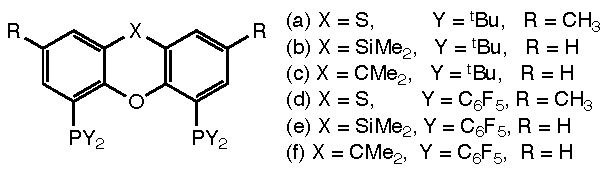
\includegraphics[]{../Figures/Proposedligands.pdf}
\caption[Proposed ligands for investigation]{Proposed ligands for investigation}
\label{Proposedligands}
\end{figure}

The coordination properties of the ligands will be investigated by formation of complexes with a range of metals including platinum, palladium, iridium and rhodium.  These late transition metals are electron-rich so will form weaker metal-oxygen bonds than the earlier and first row transition metals.  Halide complexes will be formed initially as the halide can be readily abstracted by a silver salt allowing the formation of three-coordinate complexes.  At this point the electronic properties of the complexes will be investigated by the formation of carbonyl complexes.  The carbonyl stretching frequency is commonly utilised as a measure of electron density on the metal.\cite{Tolman1977}  Measuring this frequency will allow a qualitative evaluation of the electron- withdrawing and donating properties of the ligands comparing the \emph{tert}-butyl and pentafluorophenyl ligands.  It was also be used to determine the electronic impact of altering the bridging group in the backbone between \ce{CMe2}, \ce{SiMe2} and S.  

Methyl complexes (Figure \ref{Methylcomplexes}) will be synthesised by treatment of the three-coordinate and halide complexes with a methylating agent such as dimethyl zinc or methyllithium. Investigation into the reactivity of methyl complexes with a variety of halogen and carbon based electrophiles to allow the formation of functionalised methane that could be readily converted into other compounds for use as chemical feedstocks or fuels.  
 
% including N-bromosuccinamide, bromine and methyl \emph{p}-toluenesulfonate.  Reaction with the bromine electrophiles will produce bromomethane, whilst reaction with \emph{p}-toluenesulfonate will form ethane which could be further converted \emph{via} alkane metathesis or dehydrogenation to yield the higher alkanes for use as fuels or ethene which is a useful organic starting material.  

\begin{figure}[h]  
\centering
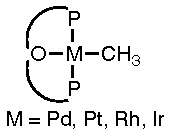
\includegraphics[]{../Figures/Methylcomplexes.pdf}
\caption[Methyl complexes]{Methyl complexes}
\label{Methylcomplexes}
\end{figure}

Further work will look at reactions of the synthesised metal complexes with alkanes focusing specifically on methane.  Upon complexation to a metal centre, the pK\sub{a} of methane decreases significantly so investigation into the reaction of various metal complexes with methane in the presence of strong bases will be carried out.  This should result in a methyl complex that can react with an appropriate electrophile \emph{in situ} to form a three-coordinate metal pincer complex and the resulting product.

Finally, the project will investigate the use of the pincer complexes for a one-pot catalytic synthesis of a useful chemical feedstock from methane.  This will involve combination of the C-H activation and electrophilic attack in the same step.

\section{Synthetic strategy}

\subsection{Ligand synthesis}

The commercially available carbon-bridged backbone will be utilised and the silicon- and sulfur-bridged backbones will be synthesised using literature methods for similar compounds.\cite{Kranenburg1995, Suter1938}  The ligands will be synthesised using a method derived from the literature for similar compounds.\cite{Kranenburg1995, Mispelaere2005}

The synthesis of the silicon bridged backbone (Scheme \ref{Siliconbackbone}) is based on that reported by Kranenburg et al.\cite{Kranenburg1995}  The synthesis involves lithiation of diphenylether at low temperature using \emph{n}-butyllithium and \gls{TMEDA} and warming to room temperature over 16 hours.  The reaction mixture is cooled to -78 \degrees C and a solution of dichlorodimethylsilane is added over one hour before stirring for 16 hours.  The reaction is quenched using water before isolation and recrystallisation from methanol.

\begin{scheme}[h]  
\centering
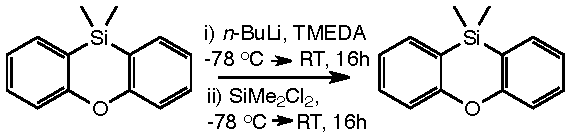
\includegraphics[]{../Schemes/Siliconbackbone.pdf}
\caption[Synthesis of the silicon bridged backbone]{Synthesis of the silicon bridged backbone}
\label{Siliconbackbone}
\end{scheme}

The sulfur bridged backbone will be synthesised by a Friedel-Crafts reaction (Scheme \ref{Sulfurbackbone}).\cite{Suter1938}  Anhydrous aluminium trichloride and sulfur are added to \emph{p}-ditolylether and heated to reflux for four hours.  The reaction is quenched with hydrochloric acid and washed with water.  The product is isolated from excess \emph{p}-ditolylether \emph{via} distillation under reduced pressure.

\begin{scheme}[h]  
\centering
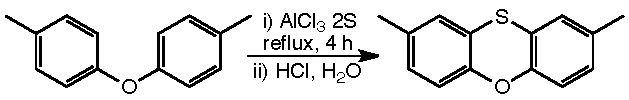
\includegraphics[]{../Schemes/Sulfurbackbone.pdf}
\caption[Synthesis of the sulfur-bridged backbone]{Synthesis of the sulfur-bridged backbone}
\label{Sulfurbackbone}
\end{scheme}

The chlorodi(pentafluorophenyl) phosphine and phosphine utilised in the ligand synthesis will be prepared as reported by Mancino et al. (Scheme \ref{Pentafluorophenyl}).\cite{Mancino2005}  The commercially available bromopentafluorobenzene will be treated with magnesium to yield a Grignard reagent.  Reaction of \ce{PCl3} with two equivalents of the Grignard reagent will yield the desired chlorodi(pentafluorophenyl) phosphine.   A similar method is already used within the research group for the synthesis of chlorodi(\emph{tert}-butyl) phosphine.

\begin{scheme}[h]  
\centering
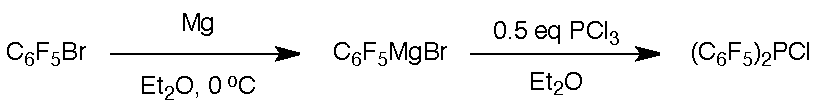
\includegraphics[width = 0.8\textwidth]{../Schemes/Pentafluorophenyl2.pdf}
\caption[Synthesis of chlorodi(pentafluorophenyl) phosphine]{Synthesis of chlorodi(pentafluorophenyl) phosphine}
\label{Pentafluorophenyl}
\end{scheme}

The synthesis of the ligands from the backbones will be the same in all cases (Scheme \ref{tBuligandsynthesis}).  The method utilised is based on combination of the reported synthesis of xantphos and the bis-(\emph{tert}-butyl-phosphino) derivative of xantphos.\cite{Kranenburg1995, Mispelaere2005}  A solution of the precusor and \gls{TMEDA} in diethyl ether will be cooled to -78 \degrees C and treated with \emph{sec}-butyllithium before warming to room temperature over 16 hours.  Upon cooling to -78 \degrees C a solution of the appropriate phosphine in diethyl ether will be added dropwise and the reaction allowed to warm to room temperature over 16 hours.  The solution will be quenched by washing with water and the product recrystallised from \emph{n}-propanol.  

\begin{scheme}[h]  
\centering
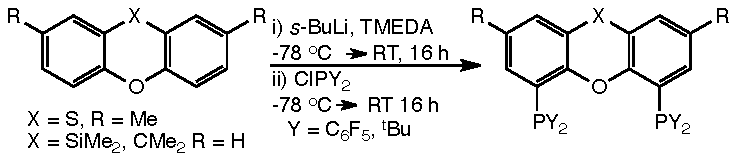
\includegraphics[]{../Schemes/tBuligandsynthesis.pdf}
\caption[Synthesis of the ligands]{Synthesis of the ligands}
\label{tBuligandsynthesis}
\end{scheme}

\subsection{Coordination complexes}

Investigations into the coordination complexes formed with the proposed ligands will focus on late second and third row transition metals, namely platinum, palladium, iridium and rhodium.  These late transition metals will form weak bonds to the oxygen centre allowing for the weakly binding methane to bond in the \emph{trans}-position.  Reactions will be carried out with metal starting materials with weakly bound ligands that can be readily replaced by the desired ligands.  As xantphos typically forms bidentate complexes, \cite{Freixa2008} it is expected that a mixture of \emph{cis} and \emph{trans} bidentate complexes will be formed initially upon reaction of the ligand with a metal halide complex (Scheme \ref{Metalcomplexes} (a)).

\begin{scheme}[h]  
\centering
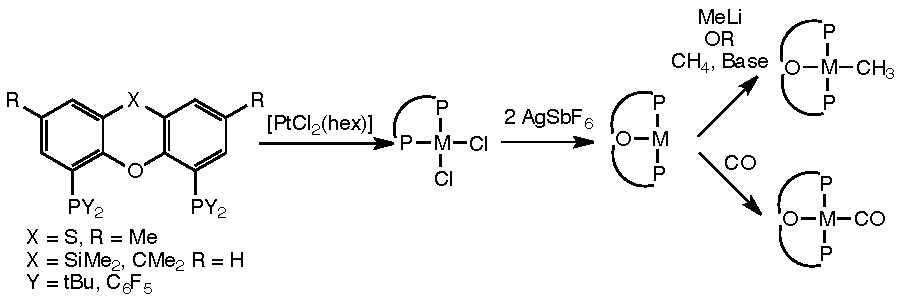
\includegraphics[]{../Schemes/Metalcomplexes.pdf}
\caption[Synthesis of the three-coordinate complexes]{Synthesis of the three coordinate complexes}
\label{Metalcomplexes}
\end{scheme}
\vspace{1cm}

Treatment of the bidentate metal halide complex with an appropriate ligand abstraction agent to remove the halide ligands will be required to promote tridentate coordination of the POP ligand.  Hence the halide complexes will be synthesised initially, as these can be treated with one or two equivalents of an appropriate silver salt, such as silver hexafluoroantimonate,  to yield the pincer coordination complex with either zero or one other ligand (Scheme \ref{Metalcomplexes} (b)).  The hexafluoroantimonate is a non-coordinating counterion so will not bond to the metal centre allowing the formation of the three-coordinate complex.  Halide abstraction under an atmosphere of carbon monoxide will allow the formation of the carbonyl complex (scheme \ref{Metalcomplexes} (c)), which will be studied using infrared spectroscopy to investigate the electronic influence of the different ligand systems.  

Upon formation of the three-coordinate complexes, treatment with a methylating agent such as dimethylzinc, methylmagnesium iodide or methyllithium will be carried out to obtain the methyl complexes (Scheme \ref{Metalcomplexes} (d)).  These complexes will be investigated for the reactive properties with a variety of electrophiles including \ce{Br2}, \emph{N}-bromosuccinamide, methyl \emph{p}-toluene sulfonate and methyl iodide.  The protonation of these complexes using acids with weakly coordinating counterions (\ce{(CF3SO2)2CHPh} and \ce{(CF3SO2)2CH2}) will be carried out in order to form $\sigma$-methane complexes which will be used to investigate the nature of the bond between the methane and the metal centre.  

Formation of the methyl complexes will also be attempted by reaction of the three-coordinate complexes with methane in the presence of a strong base (Scheme \ref{Metalcomplexes} (d)).  Upon complexation of methane, the pKa is expected to decrease similar to that found upon complexation of molecular hydrogen making deprotonation feasible.\cite{Crabtree1995}

%These methyl complexes will be reacted with a range of electrophiles to yield \fixme{bromomethane} which could be utilised as a useful chemical feedstock.

The final section of the project will investigate a combination of the C-H activation of methane to give the methyl complexes and their \emph{in situ} reaction with the electrophiles studied previously.  This will form a novel catalytic process for the formation of a useful chemical feedstock from methane.  

\section{Methodology and techniques}

All reactions will be carried out using Schlenk techniques under an inert atmosphere.  The resulting products will be characterised initially using NMR spectroscopy.  In particular \proton, \carbon~and \phosphorus~NMR, together with COSY, HSQC and HMBC experiments will be used to confirm the structural identity of the compounds.  Platinum and rhodium particularly useful as the spin 1/2, NMR active nucleus \Pt~and \ce{^{103}Rh} are 33\% and 100\% abundant.  This results in coupling of other active nuclei to the platinum, forming platinum satellites that can be used to obtain useful information about the complex.

Infrared spectroscopy will be particularly important to this project.  As oxygen NMR is not practicable, infrared spectroscopy will be utilised to distinguish between the bidentate and tridentate binding modes of the ligands.  In particular, the C-O stretch of the backbone should be readily identifiable (1243 \percm~for free xantphos\cite{Kranenburg1995}) and if the oxygen is coordinating to the metal the stretching frequency is expected to shift to lower frequency compared to both the free ligand and bidentate coordination.  Further characterisation will be carried out utilising X-ray crystallography, mass spectrometry and elemental analysis as required.  

\section{Proposed timeline}

%12 months of enrolment will be completed at 15th August 2011.

The initial six months will focus on the synthesis of the ligands.  The sulfur-bridged \emph{tert}-butyl ligand has been successfully synthesised and the synthesis of the silicon-bridged analogue has been attempted with promising results, although further work on isolation and optimisation is required.  Initially, work will focus on completing the synthesis of the silicon bridged ligand and successful synthesis of the carbon bridged ligand expecting to be completed by the end of August.  After successful synthesis of the \emph{tert}-butyl ligands the synthesis of the electron-withdrawing, pentafluorophenyl ligands will be attempted.  It is expected that the ligand synthesis stage will be completed in November 2011.

The investigation into the halide complexes and the halide abstraction to form the three-coordinate complexes will be carried out concurrently with the synthesis of the ligands.  It is expected that the  ligands will be air-sensitive, so it is important to carry out reactions of the ligands as close to the time of synthesis as possible.  However the complexes that are formed are more likely to be air-stable, so reactions of these can be carried out at a later date.

Synthesis and analysis of the carbonyl complexes and investigation into the methylation of the three-coordinate species will be carried out in early 2012, followed by the electrophilic reactions and C-H activation of methane.  The research into the catalytic reactions will be performed in early 2013.  The proposed submission date is August 2013. 

\begin{table}[h]
\caption[Proposed timeline]{Proposed timeline}
\label{Timeline}
\begin{center}
    \begin{tabular}{l l l}
    \hline
Project component					& Beginning Date 	& Completion Date	\\ \hline
\emph{tert}-butyl ligand synthesis		& In progress		& August 2011		\\
pentaflurophenyl ligand synthesis		& September 2011	& November 2011	\\
Synthesis of halide complexes			& August 2011		& December 2011	\\
Synthesis of three-coordinate complexes	& August 2011		& December 2011	\\
Synthesis of carbonyl complexes		& January 2012	& February 2012	\\
Methylation 						& March 2012		& May 2012		\\
Electrophilic reactions				& June 2012		& August 2012		\\
C-H activation of methane			& September 2012	& November 2012	\\
Catalytic investigations				& December 2012 	& March 2013		\\
Writing thesis 						& April 2013		& August 2013		\\
    \hline
    \end{tabular}
    \end{center} 
    \end{table}

%Relationship between dihydrogen and methane see Shilov 1997 pg 2881\\

%Electron rich metal\\
%	Stronger pi donation into sigma* orbital\\
%	Results in decreased bond order and cleavage of the bond\\
%	Oxygen very weak ligand on Pt  so would promote formation of a stronger bond trans to it\\
	
%Moulton 1976\\
%	Di-t-butylphosphines promote hydride formation, internal C- or O-metallation and co-ordinative unsaturation, stabilse unusual valence states such as Ir(II) or unusual compounds such as Pt dihydrides\\
	
%Zhu 2008: see conclusion for the impact of trans influence on C-H activation\\

%Synthesis of ethane or ethene from methane
	
%	The poor activity of pincer complexes compared to complexes with monodentate phosphine suggests that phosphine loss or rearrangement may be necessary for beta-elimination by the alkyl hydride intermediate.\cite{Wang1996}
	
%Activation of the methane under basic conditions.  Upon complexation of hydrogen with metals the pKa is reduced from 35 to 0-15.\cite{Crabtree2001}  The pKa of methane is 40/56 depending on source (40 from Crabtree1995\cite{Crabtree1995} 56 from Bordwell1988\cite{Bordwell1988}) pKa of various compounds in DMSO is given in table \ref{pKatable}

%\begin{table}[h]
%\caption[pKa's of various compounds]{pKa's of various compounds}
%\label{pKatable}
%\begin{center}
    %\begin{tabular}{l l l l}
    %\hline
%Compound 			& pKa 	& Reference\\ \hline
%Hydrogen 			& 35 		& \cite{Crabtree2001}\\
%Complexed Hydrogen 	& 0 - 15	& \cite{Crabtree2001}\\
%Methane				& 40 / 56  	& \cite{Bordwell1988}\\
%Xanthene				& 30		& \cite{Bordwell1988}\\
%Thioxanthene			& 28.6	& \cite{Bordwell1988}\\
%$^t$BuLi				& 53		& \cite{Bordwell1988}\\
%KO$^t$Bu				& 18		& \cite{Bordwell1988}\\
%LDA					& 36		& \cite{Bordwell1988}\\
    %\hline
    %\end{tabular}
    %\end{center} 
    %\end{table}

%Reaction under argon to prevent competitive binding of nitrogen\\
%Activation of methane under fischer-porter bottle synthesis\\
%Methyl complex may be too stable to undergo functionalisation i.e. will the methyl have orbitals / electron
%density available to donate / be donated into\\
%Possibility of using a source of Cl+ to react with the complexed methyl to form \ce{CH3Cl}\\
%Or using \ce{Br2}? better than chlorine gas\\
%Issue that the product may be more reactive towards the complex\\
%\ce{CH3Cl} bp = -24.2 \degrees C so will be a gas at RT\\
%\ce{CH3Br} bp = 3.56 \degrees C\\
%\ce{CH4} bp = -161.6 \degrees C\\
%Methane boils much lower so could use dry ice/acetone trap to condense the product from excess methane and collect excess methane in liquid \ce{N2} trap\\
%Rather than using a base use a borane to form the boron compound which could then react somehow\\



%The proposed research will not involve any animal or human subjects or tissues nor is not expected to impact  people's privacy, rights or freedoms and as such ethics approval is not required.

%Schlenk working under argon rather than nitrogen to prevent competitive binding\\
%Fischer-porter bottles?\\
%NMR (1D, \proton, \carbon, \phosphorus, 2D, HSQC, HMBC etc)\\
%Platinum as an NMR active nuclei\\
%IR (C-O bond stretch changes on coordination)\\
%X-Ray crystallography\\
%Mass spec\\
%Elemental analysis\\

